\chapter{Feed Forward Neural Network}
\section{Introduction}
The \textbf{Feed Forward Neural Network} (FFNN) is a particular type of neural
network where each layer is connected to the next one without loop. We can think
at each layer as a vector to a vector function.

Each layer is composed by a set of neurons, where each neuron receives a set of input
from many others, unit and computes its own activation rule.

We can think at a FFNN as a composition of many functions, where each function is
a layer. For example: if a FFNN try to approximate a function $f(x)$ and has $3$
hidden layer, we can represent it as:
\begin{equation*}
    f(x) = f^3(f^2(f^1(x)))
\end{equation*}
where $f^i$ is a function of $i$-layer. The overall length of hidden layers is
the \textbf{depth} of the model.

During the training process we want to learn a function $f(x)$ that, starting from
the training data, try to approximate the \textbf{target function} $f^*(x)$.

In the case of supervised problems, each instance $x$ is associated with a label
$y\sim f^*(x)$, therefore, the output layer at each point $x$ must produce a value
that is close to $y$.
\begin{note}
    It's important that is $y \sim f^*(x)$ and not $y=f^*(x)$ because we want a
    model that generalizes.
\end{note}

The behavior of the intermediate layers (\textbf{hidden layers}) are not directly
specified by the training data, but is the learning algorithm that must decide
how to use these layers to best implement an approximation of $f^*$. The dimensionality
of the hidden layers is called \textbf{width} of the model.

\subsection{Training process}
The training process can be summarized as follows: initially, the network's weights
are randomly initialized. Then, for each training example $(x, y)$, the network
computes $f^\ast(x)$. Next the error $E(y, f^*(x))$ is calculated, and all weights
are adjusted using the gradient approximate, which is calculated with \textbf{backpropagation}.

\begin{note}
    During the training phase, the weights are adjusted every $n$ examples,
    where $n$ is the batch size. Weights are usually fixed by considering the
    elements of a batch to avoid overfitting.
\end{note}
\section{Weight Learning}
If $f(x)$ is \textbf{non-linear} function, twe can theoretically approximate it
using a hidden layer. The challenge lies in finding the right weights.

The essence of supervised machine learning is the creation of functions that can
analyze examples (instances) and produce generalizations (predict unseen data).
This involves searching over all possible functions, a task that is inherently
complex. To make this manageable, we typically restrict the set of all possible
functions to specific families, referred to as \textbf{hypothesis classes}.

One strategy to solve non-linear problem using a linear model is to use a
transformation of the input space. By modifying the data representation,, we can
apply \textbf{non-linear transformation} ($\phi$) to the inputs. In other words,
given an instance $x$, $\phi(x)$ represents a new set of features describing $x$.

There are several way to define a transformation:
\begin{itemize}
    \item Use a predefine $\phi$ called \textbf{kernel}
    \item Define manually $\phi$ but it isn't convenient.
    \item We can learn it but it isn't a general transformation. This is the
          approach used in deep learning.
\end{itemize}

In deep learning the goal is to learn the transformation $\phi$, whereas SVM use
a predefine \textit{kernel}. So, we can describe this approach using the
following model:
\begin{equation}
    f(x, \theta, \omega) = \phi(x; \theta)^T \cdot \omega
\end{equation}
Here, $\theta$ represents the parameters used to learn the transformation $\phi$
from a broad class of functions, while $\omega$ represents the parameters mapping
$\phi(x)$ to the target.

\begin{note}
    In a deep learning model, $\phi$ defines a hidden layer.
\end{note}

The prediction model is typically a high dimensional linear function, $f(x): x \cdot W + b$.
Below are some examples:
\begin{itemize}
    \item \textbf{Sign function}: this function is used for binary classification:
          \begin{equation}
              \hat{y} = sign(f(x))
          \end{equation}
    \item \textbf{Sigmoid function}: Used for binary classification when confidence
          in decisions is required, such as in log-linear binary classification:
          \begin{equation}
              \hat{y} = \frac{1}{1+e^{-f(x)}}
          \end{equation}
    \item \textbf{Softmax}: this is used for multi-class classification, suppose
          to have $k$ classes:
          \begin{equation}
              \hat{y} = softmax(f'(x)) = \frac{e^{f'(x)_i}}{\sum_{j=1}^k e^{f'(x)_j}}
          \end{equation}
\end{itemize}

\textbf{Pros} for linear models are that can be fit efficiently and reliably, because
gradient on linear model are easy to compute.

\textbf{Cons} models are restricted to linear functions so they works for data linear
separable, solved by a transformation.
\section{Kernel trick}
Transform the input space into an higher-dimensional space can be useful to solve
non-linear separable problem. However, this approach increase the number of
parameters and the complexity of the model. To address this challenge, we can map
the input space into a higher-dimensional space using specific functions called
\textbf{kernels}.

\begin{note}
    There can be many transformations that allow the data to be linearly separated
    in higher dimensions, but not all of these functions qualify as kernels.
\end{note}

This approach is functional because we can use the \textbf{kernel trick} to operate
in the original feature space without computing the coordinates of the data in a
higher-dimensional space.

A general linear model would be rewritten as:
\begin{equation}
    \omega^T x + b = b+ \sum_{i=1}^m \alpha_ix^Tx^{(i)}
\end{equation}
where $b$ is the bayes, $\alpha_i$ is a coefficient, $x$ is a point, $x^{(i)}$ is
$i$-th instance of training set and $m$ is the number of training instances.

To apply this model on non-linear separable data, we introduce a transformations
$\phi$ to the input space, resulting in:
\begin{equation}
    f(x) = \omega^T \cdot x + b = b + \sum_{i = 1}^m \alpha_ix^Tx^{(i)} = b +
    \sum_{i=1}^m \alpha_i\phi (x^T) \cdot \phi(x^{(i)})
\end{equation}
The kernel trick override $\phi(x^T) \cdot \phi(x^{(i)})$ with $k(x^T, x^{(i)})$,
where $K(\cdot , \cdot)$ is the kernel function. This eliminates the need to
compute $\phi(x)$ directly, making it computationally more efficient.

Furthermore, kernel trick allows us to learn models that are non-linear functions
of $x$ using a convex optimization techniques, which are guaranteed to converge
efficiently. This is possible because $\phi $ is fixed, and we optimize only the
coefficient $\alpha_i$. In Support Vector Machines (SVMs), only support vectors
are used in the model, and $\alpha_i= 0$ if and only if $i$ is not a support vector.

Any algorithm that uses kernel is called \textbf{kernel machines} or \textbf{kernel
    methods}
\section{Gradient optimization}
In deep learning, we aim to minimize the \textbf{loss function}, which, in the
context of optimization, is referred to as the \textbf{objective function}. To
achieve this, we use partial derivatives $\frac{\delta}{\delta x_i} f(x)$ to
measure how the loss function changes when only the variable $x_i$ is varied.

The \textbf{gradient} $\nabla f(x)$ generalizes the concept of derivative to
higher dimensions. In other word, the gradient is a vector where the $i$-th element
represents the partial derivative of the function with respect to $x_i$.

To minimize the loss function, we move in the direction opposite to the gradient.
This approach, known as \textbf{gradient descent}, is defined as:
\begin{equation}
    x' = x - \eta \nabla f(x)
\end{equation}
where $x$ is the current point, $x'$ is the updated point, $\eta$ is the learning
rate and $\nabla f(x)$ is the gradient of the loss function.

\begin{note}
    The gradient descent converge when every element of the gradient is zero.
\end{note}

The learning rete is an hyperparameter that controls the step size in the gradient's
direction. The optimal value of $\eta$ may change during the training, but do to
computational cost, it is often kept fixed. A good strategy involves starting with
a high learning rate to explore different paths and reduce the likelihood of
getting stuck in a local minimum, and then gradually decreasing it to converge
to the global minimum.

Since in many loss function are not convex, they cannot be optimized in a close
form. Instead, we use iterative numerical optimization method to find the minimum
of the loss function. An example is \textbf{gradient descent}.

In some cases, evaluating the loss function directly may be computationally
expensive. However, as long as we can approximate the gradient, iterative
numerical methods can still be applied.

Since the goal of our network is to approximate a target function, we need to
measure the difference between the predicted function, that we have learned, and
the target function using a \textbf{loss function}.

Formally, this function $\mathcal{L}(\hat{y}, y)$ return a scalar value that
quantifies how well the prediction $\hat{y}$ matches the target $y$. To minimize
the optimization problem over training sample, we include the parameters of the
model $\theta$ to the loss function:
\begin{equation}
    J(\theta) = \frac{1}{n} \sum_{i=1}^n \mathcal{L}(\hat{y}_i; y_i; \theta)
\end{equation}
where $n$ is the number of training samples.

The main objective of the training algorithm is to find the optimal set of
parameters $\theta$ that minimize the loss function. Formally, this can be written
as:
\begin{equation}
    \hat{\theta} = \argmin_{\theta} J(\theta) = \argmin_{\theta} \frac{1}{n}
    \sum_{i=1}^n \mathcal{L}(\hat{y}_i; y_i; \theta)
\end{equation}

To reduce the risk of overfitting, a \textbf{regularization term} can be added
to the loss function:
\begin{equation}
    \hat{\theta} = \argmin_{\theta} \frac{1}{n} \sum_{i=1}^n \mathcal{L}(\hat{y}_i; y_i; \theta)
    + \lambda R(\theta)
\end{equation}
where $\lambda$ is an hyperparameter that balances the trade-off between bias and
variance, and $R(\theta)$ is the \textbf{regularization term}, a scalar that
reflecting the model complexity. he regularization term discourages the model from
fitting the noise in the training data. This term does not always appear in the
loss function, but we can apply it implicitly by changing the network architecture
or altering the data. Examples of these operations are:
\begin{itemize}
    \item Disable some connections in the network.
    \item Add noise to the input data.
\end{itemize}
\begin{note}
    Networks with smaller weights tend to generalize better than those with larger
    weights. This is because noise in the input data has a more significant impact
    on networks with large weights.
\end{note}
\subsection{Stochastic Gradient Descent}
The \textbf{Stochastic Gradient Descent} (SGD) is a variant of the gradient descent
algorithm that is used to train neural networks. The computational cost of computing
the gradient of the loss function for the entire training dataset is $\mathcal{O}(n)$,
where $n$ is the number of training examples. To reduce this cost, SGD approximates
the gradient by computing it on a subset of the training data.

In its simplest form, SGD updates the model parameters after computing the gradient
on a single training example (known as \textbf{Online Learning}). While this approach
can lead to faster updates, it often results in slow convergence and noisy gradients.

To address these issues, a \textbf{mini-batch} approach is commonly used. A mini-batch
is a small, randomly selected subset of the training data, typically ranging from
1 to a few hundred examples. By computing the gradient on a mini-batch, the
algorithm achieves a balance between convergence stability and computational
efficiency.

We can compute the gradient of the loss function on the mini-batch as follows:
\begin{equation}
    g = \frac{1}{m} \sum_{i = 1}^{m} \nabla_{\theta} \mathcal{L}(\hat{y}_i, y_i, \theta)
\end{equation}
where $m$ is the size of the mini-batch, $\hat{y}^i$ and $y^i$ are the predicted
and actual labels for the $i$-th training example, respectively, and $\nabla_{\theta}
    \mathcal{L}(\hat{y}_i, y_i, \theta)$ is the gradient of the loss function with
respect to the model parameters $\theta$.

The model parameters are then updated as follows:
\begin{equation}
    \theta = \theta - \eta g
\end{equation}
where $\eta$ is the learning rate, and $g$ is the gradient computed on the mini-batch.

When we choose the mini-batch size, we have to consider the trade-off between
the computational efficiency and the convergence speed. In general, the larger
the mini-batch size, the more accurate the estimate of the gradient, but the
slower the convergence. While the smaller the mini-batch size, the noisier the
estimate of the gradient, but the faster the convergence.
\section{Loss/Cost function}
\begin{definition}[Loss function]
    A \textbf{loss function} maps the outcome of a single data point, represented
    by one or more variables, to a real number. This number intuitively reflects
    the network's performance on that specific data point.
\end{definition}
\begin{definition}[Cost function]
    A \textbf{cost function} maps the average loss over an entire dataset to a
    real number, representing the overall performance of the model.

    A cost function should align with the intended purpose of the network to
    ensure effective optimization.
\end{definition}
With these definitions, we can state that the goal of a training algorithm is to
minimize the cost function. Lower values of the cost function generally indicate
better network performance.

There is a wide range of loss functions that can be used in deep learning, so we
need to choose the right one for our problem. The choice of a loss function depends
on the specific task the model is intended to solve. Below are common examples of
loss functions for classification and regression tasks.
\paragraph{Classification loss functions}
\begin{itemize}
    \item \textbf{Maximum likelihood}: this approach optimizes the likelihood of
          the model's predictions matching the target distribution:
          \begin{equation}
              \mathcal{L} = - \frac{1}{N} \sum_{i=1}^N y_i p(\hat{y}_i) +
              (1-y_i) p(1-\hat{y}_i)
          \end{equation}
    \item \textbf{Binary Cross-entropy (log-loss)}: Used for binary classification tasks:
          \begin{equation}
              \mathcal{L} = - \frac{1}{N} \sum_{i=1}^N y_i \log(p(\hat{y}_i))
              + (1-y_i) \log(p(1-\hat{y}_i))
          \end{equation}
    \item \textbf{Categorical Cross-entropy}: Suitable for multi-class classification problems:
          \begin{equation}
              \mathcal{L} = - \sum_{i=1}^N y_i \log(p(\hat{y}_{i}))
          \end{equation}
\end{itemize}
\paragraph{Regression loss functions}
\begin{itemize}
    \item \textbf{Mean Squared Error}: Measures the average squared difference
          between the predicted and actual values:
          \begin{equation}
              \mathcal{L} = \frac{1}{N} \sum_{i=1}^N (y_i - \hat{y}_i)^2
          \end{equation}
    \item \textbf{Mean Absolute Error}: Measures the average absolute difference
          between predictions and targets:
          \begin{equation}
              \mathcal{L} = \frac{1}{N} \sum_{i=1}^N |y_i - \hat{y}_i|
          \end{equation}
    \item \textbf{Huber Loss}: Combines the properties of MSE and MAE to handle
          outliers effectively:
          \begin{equation}
              \mathcal{L} = \frac{1}{N} \sum_{i=1}^N \begin{cases}
                  \frac{1}{2}(y_i - \hat{y}_i)^2                  & \text{if } |y_i - \hat{y}_i| \leq \delta \\
                  \delta |y_i - \hat{y}_i| - \frac{1}{2} \delta^2 & \text{otherwise}
              \end{cases}
          \end{equation}
\end{itemize}
\begin{note}
    The list above is not exhaustive; many other loss functions exist for specialized
    tasks.

    It is possible to define custom loss functions. In such cases, it is crucial
    that the function is differentiable, as this ensures compatibility with
    gradient-based optimization methods.
\end{note}
\section{Output function}
The choice of the loss function is closely related to the choice of the \textbf{
    output unit}, which is the final layer of a neural network. The output unit
is responsible for transforming the features generated by the network into the
appropriate format for the task at hand.

There are many output units that can be used in deep learning, here are some examples:
\begin{itemize}
    \item Linear;
    \item Sigmoid;
    \item Softmax;
    \item Gaussian Mixtures;
\end{itemize}
\subsection{Linear output unit}
One simple output unit is the linear unit, which is based on linear model:
\begin{equation}
    \hat{y} = W^T \cdot h + b
\end{equation}
where $W$ and $b$ are the learnable weights and bias, and $h$ represents the features
from the previous layer.

Linear output units are typically used in regression tasks where the target variable
can take any real value. They are also used for modeling the mean of a Gaussian
distribution. However, they are unsuitable for classification problems, as they
do not constrain the output to a specific range, such as probabilities.
\subsection{Sigmoid output unit}
The sigmoid output unit is used for binary classification task. The output
of this unit is a value between $0$ and $1$ and it can be interpreted as the
probability of the input belonging to the positive class.

This function can be approximated using the linear output unit, but the function
we create would have 0 gradient outside the $[0, 1]$ range, so the learning
algorithm would not be able to update the weights.

The sigmoid function resolve the previous problem, because it ensure a strong
gradient whenever the model has a wrong answer. The sigmoid function is defined as:
\begin{equation}
    \sigma(x) = \frac{1}{1+e^{-x}}
\end{equation}
\subsection{Softmax output unit}
The softmax output unit is used for multi-class classification tasks. It produces
a probability distribution over $k$ classes, where each value indicates the likelihood
of the input belonging to a specific class. To implement this we need to have a
linear layer to predicts the un-normalized log probabilities and then we apply
the softmax function to normalize the output.

The softmax function is defined as:
\begin{equation}
    \sigma(x)_i = \frac{e^{x_i}}{\sum_{j=1}^k e^{x_j}}
\end{equation}
where $x_i$ is the unnormalized log probability for the $i$-th class.

The softmax function is a good output function because is continuous and
differentiable.

It preserves the relative order of the input values, ensuring that the class with
the highest log probability remains the most likely after normalization.

The output of the softmax function can be interpreted as the probability of the
input belonging to each class. However, the model may overfit to known classes,
potentially misclassifying inputs from unknown or unseen classes with high confidence.
\subsection{Gaussian Mixtures output unit}
In some cases, we need to perform multimodal regression, where the target variable
$y$ is drawn from a conditional distribution $p(y|x)$ that exhibits multiple peaks
for the same input $x$.

To model such distributions, we can use a \textbf{Gaussian Mixture Model} (GMM),
defined as:
\begin{equation}
    p(y|x) = \sum_{i=1}^n p(c= i|x) N(y; \mu^{(i)}(x), \Sigma^{(i)}(x))
\end{equation}
where the Neural network output have the following value:
\begin{itemize}
    \item $p(c=i|x)$ is the mixture component, representing the probability of
          selecting the $i$-th Gaussian.
    \item $\mu^{(i)}(x)$ is the mean of the $i$-th component.
    \item $\Sigma^{(i)}(x)$ is the covariance matrix of the $i$-th component.
\end{itemize}
\section{Activation Function}
The \textbf{hidden unit} applies an affine linear transformation such as:
\begin{equation}
    z = Wx + b
\end{equation}
where $W$ is the weight matrix, $x$ is the input vector and $b$ is the bias vector.
On the results of this transformation, we apply a non-linear function called
\textbf{activation function}.

\subsection{Tanh}
Hyperbolic Tangent is similar to sigmoidal function. The main difference between
them is that, the negative input are mapped in strongly negative value and zero
inputs are mapped in zero.

Some important characteristics are that the $\tanh$ is \textbf{differentiable}
and \textbf{monotonic}, but its derivative isn't \textbf{monotonic}.
\begin{note}
    The $\tanh$ function is used for \textbf{binary classification} problems.
\end{note}

Cause the form of the derivative values, which are greater than sigmoidal's derivative,
this function can help to speed up the training phase.
\subsection{Rectified Linear Unit}
Rectified Linear Unit (ReLU) is the most used activation function in neural networks.
This function is described as:
\begin{equation}
    g(x) = \max[0,z]
\end{equation}
We can see that ReLU is differentiable anywhere at the point where the value is
$0$. This is not a problem since we compute the gradient using approximation an
the probability to get $0$ is low.

ReLU allows us to simplify the model because we can get a sparse representation
of the network, due the possibility to deactivate some neurons. This is possible
thanks to negative input which will be converted to zero so it will be deactivated.

Since ReLU have a ``problem'' with the $0$ value, there are some generalization
that can be used to solve this. In order to do this, we can express the ReLU as
a generalization of the following formula:
\begin{equation}
    h_i = g_i(z,\alpha) = max(0,z_i) + \alpha_i min(0, z_i)
\end{equation}
Other versions of ReLUs are:
\begin{itemize}
    \item \textbf{Absolute value rectification}: this function is obtained by
          fixing $\alpha_i = -1$ to express $g(z) = |z|$. It is used to object
          recognition.
    \item \textbf{Leaky ReLU}: this function is obtained by fixing $\alpha_i = 0.01$.
          This one solves the problem of zero gradient which means that the model
          doesn't learn. This is done by Leaky ReLU with a small linear component
          for negative input.
    \item \textbf{Parametric ReLU}: this function is like Leaky ReLU but the
          parameter $\alpha_i$ is learned.
    \item \textbf{Maxout units}: the activation function $f$ is learned. It
          combines different ReLU to produce a convex function.
\end{itemize}
\subsection{Softplus}
Another generalization of the ReLU function is the Softplus function. This function
is defined as:
\begin{equation}
    f(x) = \log(1+e^x)
\end{equation}
This function was defined to solve ReLU's problem of non differentiable point,
it is a smooth approximation of ReLU. Theoretically we can think to get better
performance using this function compared to ReLU, but empirically it doesn't.

\subsection{Differences}
There are some guides to use these activation functions:
\begin{itemize}
    \item Sigmoids and their combinations generally works better in case of classifiers.
    \item Sigmoids and tanh Sometimes are avoided due the vanishing gradient problem.
    \item ReLU is the default activation function for hidden layers.
    \item We can use Leaky ReLU if we encounter a case of dead neurons.
    \item ReLU should only be used for hidden layer.
\end{itemize}
In general we can initially use ReLU, than if we cannot obtain better performance
we can change activation function.
\section{Initialization}
Another important step inside the planning of a deep neural network is the
initialization process.

First of all we can initialize all \textbf{bias} to $0$ to discover eventually
dead neurons. % ?

For \textbf{weights} we must not initialize to the same values because we have to
brake the symmetry of the model, so we can sample weights from a normal
distribution with mean $0$ and variance dependant of the number of neurons in
the previous layer.
\begin{equation*}
    W^{[l]} \sim \mathcal{N}\left(0, \frac{1}{n^{[l-1]}}\right)
\end{equation*}
\section{Regularization}
Regularization is a technique used to prevent overfitting. In the context of
deep learning, most regularization strategies are based on \textbf{regularizing
    estimators}. This is done through reducing variance at the expense of
increasing the bias of the estimator. In the following, we are going to see some
regularization techniques.

Here we can see a list of all techniques:
\begin{itemize}
    \item Parameters norm penalties
    \item Dataset augmentation
    \item Noise robustness
    \item Early stopping
    \item Parameter tying and parameter sharing
    \item Multitask learning
    \item Bagging and other ensemble methods
    \item Dropout
    \item Adversarial training
\end{itemize}

We need to have a model that is capable to generalize on unseen data, so we have
to find the right trade-off in order to avoid overfitting and underfitting.

In the context of deep learning, most regularization strategies are based on
\textbf{regularizing estimators}. This is done through reducing \textbf{variance}
and increasing \textbf{bias} of the estimator.
\begin{note}
    A good estimator is one that decreases the variance without increasing too
    much the bias.
\end{note}

When we are working with deep learning to solve complex tasks, we can encounter
different problems. This can increase the complexity of the model and the risk of
overfitting. In this case, we can find the best large model and in the end apply
a regularization process to reduce the complexity of the model and improve the
generalization.

The idea behind regularization is to train a model that does not simply minimize
the loss function, but also manages the variability of the data. To achieve this
goal, we can use one of the following techniques:
\begin{itemize}
    \item \textbf{Directly}: introducing prior knowledge or express generic
          preference for a simpler model class. This is implemented by changing
          constraints, adding restrictions on the parameter values or changing
          objective function. The constraints serve to penalize certain values
          of the parameters.
    \item \textbf{Undirectly}: in this case we are not manipulating the model but
          we are changing the training data. This can be done using technique
          such as data augmentation, introducing noise in the training data or
          using ensemble methods.
\end{itemize}
\subsection{Regularization strategies}
\subsubsection{Parameters Norm Penalties}
The most traditional form of regularization consists in adding a penalty to the
objective function. This can be done by modifying the loss function as follows:
\begin{equation}
    \hat{J}(\theta) = J(\theta) + \alpha \Omega(\theta)
\end{equation}
where $\alpha \in [0, \infty)$ is a hyperparameter that regulates the contribution
of the norm penalties. This parameter can change for each layer.

Since we have added a penalty term, the optimizer will try to minimize the loss
function and at the same time it decreases some measure of the size of the
parameters $\theta$. It affects only a subset of parameters.

$\Omega$ usually penalizes only the weights ($W$) of the affine transformation
at each layer, not the bias ($b$).

This method can be implemented using different norms, here we can see some of them:
\begin{itemize}
    \item \textbf{Sum of the weights} ($L_1$): pushes all values to $0$ penalizing
          small weights more than big one.
          \begin{equation}
              \Omega(w) = \sum_{w_j}|w_j| = \|w\|_1
          \end{equation}
    \item \textbf{Sum of the squared weights} ($L_2$): penalizes large values more:
          \begin{equation}
              \Omega(w) = \sum_{w_j}|w_j|^2 = \|w\|_2
          \end{equation}
    \item \textbf{$p$-norm} ($L_p$): for $p<2$ encourage sparser vector, while
          larger values of $p$ discourage large weights more:
          \begin{equation}
              \Omega(w) = \sqrt[p]{\sum_{w_j}|w_j|^p} = \|w\|_p
          \end{equation}
          In general, all the $p-$norms are used to penalize large weights more
          than small ones.
\end{itemize}

The effect of the $L_2$ norm is to shrinks weights on features that add noise to
the model (feature with high variance but low covariance with target), while
$L_1$ norm provides a solution that is sparse. This property can be seen as a
features selection mechanism.
\begin{note}
    Using $L_2$ negative and positive weights moves towards 0 depending on the
    magnitude of the weights, while using $L_1$ negative and positive weights
    moves towards 0 regardless of magnitude.
\end{note}

Another improve that we can add to the previous model are constraints related to
regularization term, for example, if we consider the following loss function:
\begin{equation}
    \hat{J}(\theta) = J(\theta) + \alpha \Omega(\theta)
\end{equation}
we can add a constraint to the regularization term as follows:
\begin{equation}
    \Omega(\theta) \le k
\end{equation}
where $k$ is a small value.

In this way the optimization problem changed because we have to consider also
the upper-bound of regularization term.

To solve this problem, we can construct a generalize \textbf{Lagrange function},
consisting of the original objective function plus a set of penalties. Each
penalty is a product between a coefficient, called a Lagrange multiplier ($\alpha$),
and a function representing whether the constraint is satisfied.
\begin{equation}
    \mathcal{L}(\theta, \alpha; X,y) = J(w;X,y)+ \alpha(\Omega(\theta)-k)
\end{equation}
Formally the optimization problem will be:
\begin{equation}
    \argmin_\theta \max_{\alpha \geq 0} \mathcal{L}(\theta, \alpha)
\end{equation}

To solve this problem we can use techniques that minimize $J$ and then project
the solution obtained to the feasible region $\Omega(\theta) - k$. This method
prevent to get stuck in local minimum and impose stability on the optimization
procedure.
\subsubsection{Dataset augmentation}
We can get better generalization training model on more data. The main problem is
that data is limited also labelling is an extremely tedious task. \textbf{Dataset
    augmentation} provides a cheap easy way to increase the amount of your
training data.

Moreover, when you are comparing different algorithms you have to compare on
augmented and non augmented dataset to avoid bias.

To implement this technique exists a lot of algorithms, but when we use this
we need to be careful to not introduce bias in the dataset or altering the output.
\subsubsection{Noise robustness}
\textbf{Noise injection} can be thought of as a form of regularization. When we
add a noise with infinitesimal variance at input of the model is equivalent to
imposing a penalty on the norm of the weights.

Noise can be injected at different levels of deep models, if we add on input we
are defining a data augmentation procedure, so we have to use some of the best
practices explained before.

Adding small noise pushes model into regions where the model is insensitive to
small variations in weights, finding points that are not merely minima, but
minima surrounded by flat regions.

Since some dataset present mistake on the labels, we can remedy this problem by
adding noise to the labels. This can be done through setting a probability $\varepsilon$
for which we think the labels are correct.

This method implemented analytically in the \textbf{cross entropy} function.
Another example of this technique is \textbf{label smoothing}, where we use
softmax activation function in the output layer to get a probability.
\begin{equation*}
    \left[\begin{array}{c}
            1 \\0\\\vdots\\ 0
        \end{array}\right]_{label} \implies \left[\begin{array}{c}
            0.9 \\0.01\\\vdots\\ 0.02
        \end{array}\right]_{label}
\end{equation*}

Using a softmax we will never predict 0 or 1 but it will predict a probability so
model can always learn and make more extreme prediction forever. This has the
advantage of preventing the pursuit of hard probabilities without discouraging
correct classification.
\subsubsection{Multitasking learning}
\textbf{Multitasking learning} is a way to improve generalization by pooling the
examples arising out of several tasks. It is usually performed through the
following architecture:
\begin{itemize}
    \item \textit{Task-specific parameters}: which only benefit from the examples
          of their task to achieve good generalization.
    \item \textit{Generic parameters}: parameters shared across all tasks which
          benefit from the pooled data of all tasks.
\end{itemize}
\begin{figure}[!ht]
    \centering
    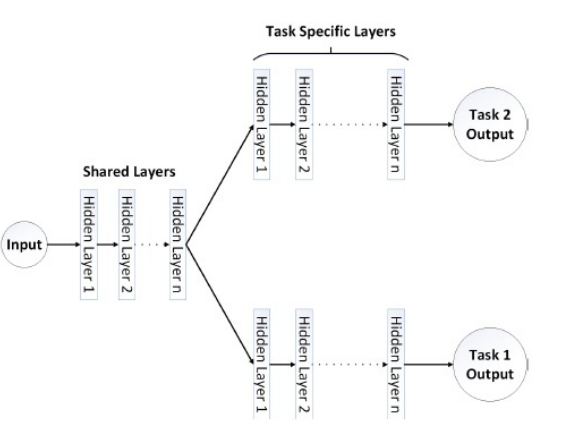
\includegraphics[width=0.5\textwidth]{img/multitask.png}
    \caption{Multitasking learning}
    \label{fig:multitask}
\end{figure}
\begin{note}
    Multitasking learning is a form of parameter sharing.
\end{note}

Shared parameters improve generalization in proportion of number of examples for
the general task. Additional task imposes constraints on the parameters in the
shared layers preventing overfitting.
\begin{note}
    Improvement in generalization only occurs when there is something shared across
    the tasks at hand.
\end{note}
\subsubsection{Early stopping}
When training large models with sufficient representational capacity to overfit
the task, we often observe that training error decreases over time but validation
error begins to rise again. We can obtain a model with better validation error by
returning to the parameter setting at the point in time with the lowest validation
error.

\textbf{Early stopping} is one of the most common techniques used. We can think
at this technique as a hyperparameter selection method, where training time is
the hyperparameter to be chosen.

Early stopping can be implemented as follow:
\begin{itemize}
    \item Choose number of iterations $n$
    \item Train model for $n$ iterations
    \item Validate model and compute validation error, compare consecutive validation
          error and return to point 2 until delta is insignificant or negative.
\end{itemize}
Every iteration model improves its weights until it starts to going in overfitting.
\begin{note}
    It's impossible to write all parameters on disk during training.
\end{note}
\begin{figure}[!ht]
    \centering
    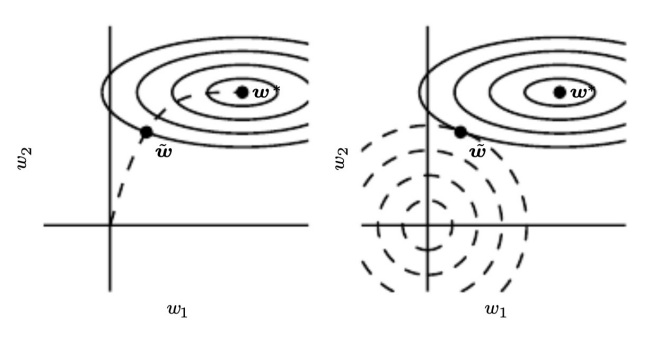
\includegraphics[width=1\textwidth]{img/early_stopping.png}
    \caption{On the left we can see the process of early stopping, while on the
        right we can see a classic regularization process.}
    \label{fig:earlystopping}
\end{figure}
\subsubsection{Parameters Tying}
\textbf{Parameters Tying} refers to explicitly forcing the parameters of 2 models
to be close to each other using the norm penalty:
\begin{equation}
    \|w(A)- w(b)\|
\end{equation}
with $A$ and $B$ respectively first and second model. This norm penalty is added
to the objective function like a constraint. It is used in Siamese networks,
convolution operators and multitasking learning.
\subsubsection{Bagging}
\textbf{Bagging} is a technique for reducing generalization error combining
several models (\textbf{ensemble model}).

You have to train $k$ different models on $k$ different subsets of training data
with same number of examples as original dataset using a random sampling with
replacement.

Every model is then tested, they produce $k$ votes for the final result. These
models are called ensemble.

The objective of this method is to introduce generalization by using different
models trained on different examples using different initialization hyperparameter
and different structures to have independent errors.

Cons of this method is that ensemble models doesn't provide us a scalable way to
improve performance, moreover we have 2-3 models inside the ensemble.
\subsubsection{Dropout}
\textbf{Dropout} provides a computationally inexpensive but powerful method of
regularizing a broad family of models. It provides an inexpensive approximation
of a ensemble with a high number of sub-networks of the starting one.

All the sub-networks should be formed by removing non-output units from underlying
base network, generating an exponential number of models, using a treatable
amount of memory.

This technique eliminates the need to accumulate model votes in the inference
phase. It is intended to train the model to be learned by switching on and off
with different probabilities input neurons or neurons in the hidden layers.

To do a train phase we use a \textbf{minibatch-based learning algorithm} that
makes small steps, such as stochastic gradient descent.

Each time we change minibatch we \textbf{randomly sample} a different binary mask
to apply to all input and hidden units in the network. Typically the distribution
use for sampling is not uniform. For example, the probability of keeping a hidden
unit is $0.5$, while the probability of including an input unit is $0.8$.

We can have some problem, infact, at training time we are required to divide the
output of each unit by the probability of that unit's dropout mask, so we assign
as likelihood on the output. In this way we make sure that the expected total
input to a unit at test time is the same as the expected total input of that unit
at train time.

We haven't theoretically basis for the accuracy but empirically it perform well.
Complexity of dropout is limited to a $\mathcal{O}(n)$ computation per example
to update because it needs to generate a total of $n$ random numbers and multiply
them by the state.

Dropout can be used with every model and also with stochastic gradient descent.
The cost of applying dropout to the entire model could be significant, but the
amount of benefit on generalization error couldn't be enough to the cost of the
regularization.
\subsubsection{Adversarial training}
We can add \textbf{adversarial examples} that are perturbed examples of train
set. These are used to train the network and will allowed us to reduce test errors.

Adversarial examples can be generated by adding to a bit of perturbation on some
train example with a low multiplication factor of noise. This method allowed us
to generate new examples for training from the original train set with slightly
changes that are unrecognized by humans.
\section{Generative Adversarial Models}
\textbf{Generative Adversarial Network} (GAN) are generative model that
implicitly learn the \textbf{data distribution} from a zero-sum game between 2
computing neural network:
\begin{itemize}
    \item \textbf{Discriminator}: a neural network that classify examples between
          fake and real.
    \item \textbf{Generator}: generate fake example that are given as input to the
          discriminator.
\end{itemize}

\begin{figure}[!ht]
    \centering
    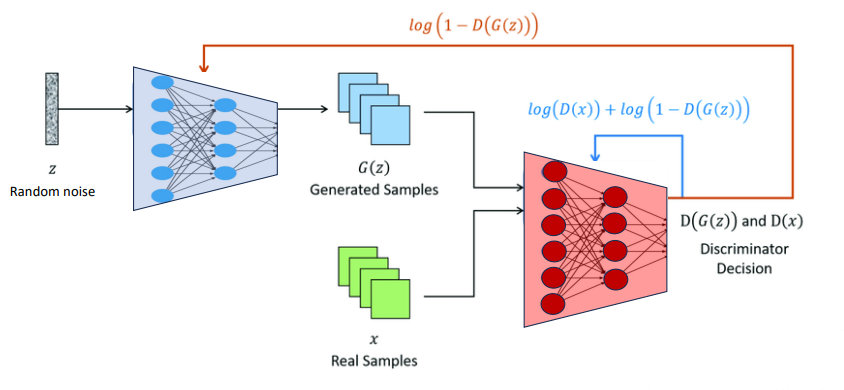
\includegraphics[width=0.5\textwidth]{img/GAN.png}
    \caption{Generative Adversarial Network}
    \label{fig:gan}
\end{figure}

The target of the generator is to generate example the most similar to real one
in such a way to be classified in real example by the discriminator. Quite the
opposite the discriminator have to identify real examples from fake one. If the
discriminator makes a mistake so we will update discriminator's weights, vice
versa we will update generator's weights.
\section{Optimization for training deep models}
When we are creating a deep learning model, we have to consider different aspects
to optimize the training process. In this section, we are going to see some
issues that can arise during the training process and how to solve them.

Let's start introducing the difference between \textbf{optimization} and
\textbf{machine learning}. In the first case, we are trying to minimize a function
acting directly on it, while in the second case we are trying to minimize a loss
function that is a proxy for the true function we want to minimize.

Using, in machine learning, we want to optimize a performance measure $P$, based
on the test set. This is done optimizing a different function $J(\theta)$ hoping
that $P$ will be optimized too.

Typically, the loss function is a simple average over the training set and can be
written as:
\begin{equation}
    J(\theta) = E_{(x, y) \approx \hat{P}_{data}} L(f(x, \theta), y)
\end{equation}
where $L$ is the loss function, $f$ is the model, $x$ is the input, $y$ is the
target and $\theta$ are the parameters of the model. Also, $\hat{P}_{data}$ is
the empirical distribution of the data.

If we know the real distribution of data $P_{data}$, we can write the loss
function, also call \textbf{risk function}, as:
\begin{equation}
    J(\theta) = E_{(x, y) \approx P_{data}} L(f(x, \theta), y)
\end{equation}
and this reduce the machine learning problem to an optimization problem.

The problem of using the empirical distribution is that the model is prone to
overfitting, because we don't have enough data to represent the real distribution.

Instead of minimizing the empirical risk, we can minimize a \textbf{surrogate
    loss function}. This function is a proxy for the true loss function and it
is easier to optimize.

Another difference is that training algorithms doesn't halt at local minima, but
when the early stopping criterion is met. This can be roughly thought of as a
way to reincorporate the true loss function in the learning process.
\subsection{Batch and Minibatch}
One aspect of machine learning algorithms that separates them from general
optimization algorithms is that the objective function usually decomposes as a
sum over the training examples. Computing this expectation exactly is very
expensive, since it requires evaluating the model on every example in the entire
dataset.

However, we can compute these expectations by randomly sampling a small number
of examples from the dataset at every iteration. This works because we are
computing an expected value and, the \textbf{standard error} of the mean estimated
from a sample of size $m$ is:
\begin{equation}
    SE(\mu) = \sqrt{VAR\left[\frac{1}{m}\sum x^{(i)}\right]} = \frac{\sigma}{\sqrt{m}}
\end{equation}
where $\sigma$ is the standard deviation of the distribution. This equation show
us that there is a less then linear relationship between the number of examples
and the standard error.

Another consideration that motivates the estimation of the gradient from a
small number of samples is the redundancy in the training set.

Optimization algorithms that use the entire training set to compute the gradient
are called \textbf{batch} or \textbf{deterministic gradient methods}. While the
ones that use a single training example for that task are called \textbf{stochastic
    gradient methods}. Most of the algorithms we use for deep learning fall
somewhere in between and they are called \textbf{minibatch} or \textbf{minibatch
    stochastic methods}.

We can see the difference between these methods in the following figure \ref{fig:batchminibatch}.
\begin{figure}[!ht]
    \centering
    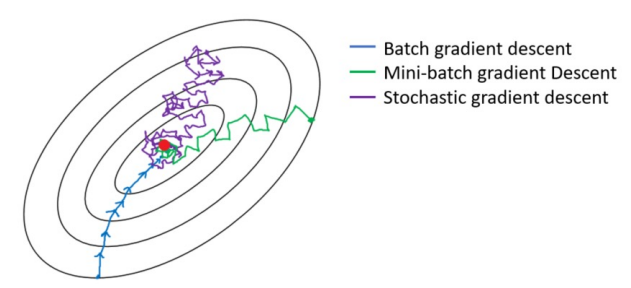
\includegraphics[width=0.5\textwidth]{img/minibatchvsbatch.png}
    \caption{Difference between batch and minibatch}
    \label{fig:batchminibatch}
\end{figure}

In order to chose the right size of the minibatch, we have to consider that a
larger size will provide a more accurate estimate of the gradient, but with less
than linear improvement in the standard error. While a smaller size will provide
a less accurate estimate of the gradient, but with more than linear improvement
in the standard error and doesn't use the full computational power of the GPU.

\begin{note}
    Usually, a good choice is a power of 2.
\end{note}

It is extremely crucial that minibatches are sampled at \textbf{random}, because
computing an unbiased estimate of the expected gradient from a set of samples
requires that those samples be independent.

When the order of elements in the dataset holds some significance, it is absolute
necessity to shuffle the examples before selecting every minibatch.
\subsection{Challenges in deep learning}
Traditionally, machine learning has avoided this difficulty by carefully designing
the objective function and constraints to insure the problem is convex. However,
for training deep models we usually face non-convex optimization.
\subsubsection{Ill-conditioning}
The first challenge is \textbf{ill-conditioning}. This is a problem that arises
when the optimization problem is poorly conditioned. This means that the curvature
of the loss function is very different in different directions.

This condition is manifested in stochastic gradient descent as a situation where
every small steps increase the loss function.

This problem can be identify by looking at the \textbf{condition number} of the
Hessian matrix. If the condition number is very large, we have an ill-conditioned
problem.
\subsubsection{Local minima}
Functions involved in deep models are guaranteed to have an extremely large
number of local minima. However, we will see that local minima are not
necessarily a major problem because flat regions are an acceptable solution.

Neural networks aren't \textbf{identifiable} there is no single set of parameters
from a single training set. Infact, if we have $m$ layers with $n$ neurons each,
there are $n!^m$ ways to arranging the hidden units to obtain equivalent solutions.
This is called \textbf{weight space symmetry}.

Model identifiability issues mean that there can be an extremely large or even
uncountably infinite amount of local minima in the cost function of deep models.
However, these local minima are all equivalent in value and are not a problematic
form of non-convexity.

Local minima are only truly problematic if they have a much higher cost than the
global minimum.
\subsubsection{Saddle points}
For many high-dimensional non-convex functions, local minima and maxima are in
fact rare compared to \textbf{saddle points}.

A saddle point is a point where the Hessian matrix has both positive and negative
eigenvalues and the gradient is zero. We can think of a saddle point as being a
local minimum along one cross-section of the cost function and a local maximum
along another.

\begin{figure}[!ht]
    \centering
    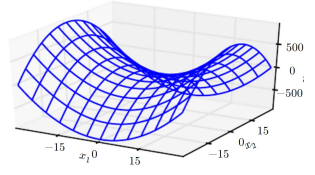
\includegraphics[width=0.5\textwidth]{img/saddle.png}
    \caption{Saddle point}
    \label{fig:saddle}
\end{figure}

This points are more common in high-dimensional spaces than local minima and they
are a problem for optimization algorithms because they are points where the gradient
is zero but they are not a minimum.

For first-order optimization algorithms that use only gradient information, the
situation is unclear. The gradient can often become very small near a saddle point.
On the other hand, gradient descent empirically seems to be able to escape saddle
points in many cases. While, for Newton's Method, saddle points constitute a
major problem, because it actively seeks solutions at critical points where the
gradient is zero.
\subsubsection{Flat regions}
Another problem that can arise during the training process is the presence of
\textbf{flat regions}. These are regions where the gradient is very small and the
optimization algorithm can't make progress.
\subsubsection{Cliffs and exploding gradients}
Neural networks with many layers often have extremely steep regions reassembling
cliffs. This regions are the result from the multiplication of many large weights
together.

An extremely steep cliff structure, the gradient update step can move the
parameters extremely far, usually jumping off of the cliff structure altogether.

A solution to this is to use the \textbf{gradient clipping heuristic} which
intervenes to reduce the step size to be small enough that it is less likely to
go outside the region where the gradient indicates the direction of approximately
steepest descent.
\subsubsection{Additional Problems}
There are other problems that can arise during the training process, such as:
\begin{itemize}
    \item \textbf{Long Term Dependencies}: arises when the computational graph
          is very deep. The result of this problem is vanishing and exploding
          gradients.
    \item \textbf{Inexact Gradients}: we usually only have a noisy or even biased
          estimate of the gradient and the Hessian. Sometimes, gradients for our
          loss functions are even intractable. Not a big issue in neural network
          training. Surrogate loss functions tend to perform well enough in practice.
    \item \textbf{Poor Correspondence between Local and Global Structure}: it is
          possible to overcome all of the above problems at a single point and
          still perform poorly if the direction that results in the most
          improvement locally does not point toward distant regions of much
          lower cost.
\end{itemize}
\begin{note}
    The initialization is very important.
\end{note}
\subsection{Optimization algorithms}
There are many optimization algorithms that can be used to train deep models.
In this section, we are going to see some of them.
\subsubsection{Stochastic Gradient Descent}
\textbf{Stochastic Gradient Descent} (SGD) is the most used optimization algorithm
in deep learning. It is based on the idea of computing the gradient of the loss
function on a minibatch and then update the weights of the model.

We can describe the algorithm as follows:
\begin{itemize}
    \item Sample a minibatch of examples from the training set.
    \item Compute the gradient of the loss function on the minibatch.
          \begin{equation}
              g \gets \frac{1}{m} \nabla_\theta \sum_{i=1}^m L(f(x^{(i)}; \theta), y^{(i)})
          \end{equation}
    \item Update the weights of the model using the gradient.
          \begin{equation}
              \theta \gets \theta - \epsilon_k g
          \end{equation}
\end{itemize}
It is important to note that the learning rate $\epsilon_k$ is a hyperparameter
that must be adaptive. This is because the learning rate is a very important
hyperparameter and it can affect the convergence of the algorithm. A sufficient
condition for convergence is:
\begin{equation*}
    \sum_{k=1}^\infty \epsilon_k = \infty \quad \text{and} \quad \sum_{k=1}^\infty \epsilon_k^2 < \infty
\end{equation*}

A common way to implement an adaptive learning rate is to use a linear decay
until the iteration $\tau$. Thi can be done as follows:
\begin{equation}
    \epsilon_k = \left(1 - \alpha\right)\epsilon_0 + \alpha \epsilon_\tau
\end{equation}
In this case we have to choose three hyperparameters: $\epsilon_0$, $\epsilon_\tau$
and $\alpha$. Usually, $\epsilon_\tau$ is chosen to be $1\%$ of $\epsilon_0$.

To choose $\epsilon_0$ we can try to make different run for a fixed number of
iterations and choose the best one.
\subsubsection{Momentum}
\textbf{Momentum} is a method that helps accelerate SGD in the relevant direction
and dampens oscillations. It is a method that accumulates an exponentially decaying
average of past gradients and continues to move in their direction.

The update rule for momentum is:
\begin{equation}
    \theta \gets \theta + v
\end{equation}
where $v$ is the velocity vector and it is defined as:
\begin{equation}
    v \gets \alpha v - \epsilon \frac{1}{m} \nabla_\theta \sum_{i=1}^m L(f(x^{(i)}; \theta), y^{(i)})
\end{equation}
where $\alpha$ is the momentum parameter and it is usually set to $0.9$.

This algorithm aims to solve the problem of poor conditioning of the Hessian
matrix, and the variance of stochastic gradients.

The momentum algorithm can be seen as a ball rolling down a hill. The ball
gathers momentum as it rolls down the hill, and it continues to move in the
direction of the momentum even if it encounters a small hill.
\subsubsection{Delta Bar Delta}
\textbf{Delta Bar Delta} is a method that adapts the learning rate for each
parameter. It is based on the following idea:
\begin{itemize}
    \item if the partial derivative of the loss function with respect to a
          parameter remains the same, increase the learning rate.
    \item otherwise, if that partial derivative changes sign, decrease
          the learning rate.
\end{itemize}
\subsubsection{AdaGrad}
\textbf{AdaGrad} is a method that adapts the learning rate for each parameter.
This method scale the gradient according to the historical norms. In this way,
learning of parameters with high partial derivatives decrease faster.

This method is based on the following idea:
\begin{itemize}
    \item Accumulate the square of the gradient into a vector $r$.
          \begin{equation}
              r \gets r + g \odot g
          \end{equation}
    \item Update the weights element wise.
          \begin{equation}
              \Delta\theta \gets - \frac{\epsilon}{\sqrt{r + \epsilon}} \odot g
          \end{equation}
    \item Update parameters
          \begin{equation}
              \theta \gets \theta + \Delta \theta
          \end{equation}
\end{itemize}
\subsubsection{RMSProp}
\textbf{RMSProp} is a method that adapts the learning rate for each parameter.
This method is a modification of AdaGrad to perform better on non-convex problems.
The main difference is that RMSProp use an exponentially weighted moving average.

This method is based on the following idea:
\begin{itemize}
    \item Accumulate the square of the gradient into a vector $r$.
          \begin{equation}
              r \gets \rho r + (1 - \rho) g \odot g
          \end{equation}
    \item Update the weights element wise.
          \begin{equation}
              \Delta \theta \gets - \frac{\epsilon}{\delta + \sqrt{r}} \odot g
          \end{equation}
    \item Update parameters
          \begin{equation}
              \theta \gets \theta + \Delta \theta
          \end{equation}
\end{itemize}
\subsubsection{Adam}
\textbf{Adam} is a variation of RMSProp in which we add the momentum. Also, it
add a bias correction to the moments to account for their initialization at the
origin.

This method is based on the following idea:
\begin{itemize}
    \item Update time step:
          \begin{equation}
              t \gets t + 1
          \end{equation}
    \item Update biased moment estimates
          \begin{equation}
              s \gets \rho_1 S + (1 - \rho_1)g \\
              r \gets \rho_2 r + (1 - \rho_2) g \odot g
          \end{equation}
    \item Correct baises
          \begin{equation}
              \hat{s} \gets \frac{S}{1 - \rho_1^t} \\
              \hat{r} \gets \frac{r}{1 - \rho_2^t}
          \end{equation}
    \item Update parameters
          \begin{equation}
              \Delta \theta \gets - \epsilon \frac{\hat{s}}{\delta + \sqrt{\hat{r}}}
          \end{equation}
    \item Update model params:
          \begin{equation}
              \theta \gets \theta + \Delta \theta
          \end{equation}
\end{itemize}